\documentclass{article}
\usepackage[preprint]{neurips_2026}

\usepackage[utf8]{inputenc}
\usepackage[T1]{fontenc}
\usepackage{hyperref}
\usepackage{url}
\usepackage{booktabs}
\usepackage{amsfonts}
\usepackage{amsmath}
\usepackage{graphicx}
\usepackage{microtype}
\usepackage{xcolor}

\makeatletter
\renewcommand{\@noticestring}{ES 678 Course Project}
\makeatother

\title{Predictive Modeling via Stacked Ensemble Learning:\\A Two-Tiered Classification Approach}

\author{%
  Meet Rajendrakumar Jain \\
  Roll Number: 26210087 \\
  ES 678 \\
  Indian Institute of Technology Gandhinagar
}

\begin{document}
\maketitle

\begin{abstract}
Tabular classification with mixed data types, missingness, and non-linear interactions often challenges single models. We investigate whether a two-level stacked ensemble using a regularized XGBoost meta-learner over five diverse base classifiers---Random Forest, Extra Trees, AdaBoost, Gradient Boosting, and an RBF-kernel SVM---improves passenger survival prediction on the Kaggle Titanic dataset ($N=891$ training, $418$ unlabeled test rows). Using a strictly leak-free preprocessing pipeline (\texttt{TitanicPreprocessor}) and aligned 5-fold stratified out-of-fold (OOF) validation, the stacked ensemble achieves 83.16\% CV accuracy (95\% bootstrap CI: [0.807, 0.856], ROC-AUC 0.8902), outperforming the default Random Forest baseline (81.14\%, McNemar $p = 0.0356$) by +2.02 percentage points and achieving the highest ROC-AUC across all models, while trailing tuned Random Forest (84.06\%) slightly on 0.5-threshold accuracy due to high base-error correlation ($r \in [0.91, 0.99]$). Diversity, regularization ablation, calibration, and SHAP analyses clarify these mechanisms.
\end{abstract}

\section{Problem and Motivation}
Predicting binary survival from passenger manifest records is a canonical tabular learning task. Let $y_i \in \{0, 1\}$ denote whether passenger $i$ survived ($1$) or perished ($0$), where one row represents one passenger aboard the RMS \textit{Titanic}. Predictions use only pre-disaster boarding attributes (class, demographics, fare, cabin, embarkation port, and family size), excluding post-event information.

Our research question is: \textit{Can a two-level stacked ensemble using regularized XGBoost over five diverse base classifiers predict passenger survival more accurately than individual models?} Tree ensembles capture axis-aligned non-linear interactions, whereas kernel SVMs learn smooth maximum-margin boundaries in scaled space. Stacked generalization \citep{wolpert1992stacked} can combine these inductive biases to improve calibration and reduce variance. We scope our claim strictly to predictive association on this historical manifest, not causal survival inference.

\section{Data and Preparation}
We use the Kaggle \textit{Titanic: Machine Learning from Disaster} dataset ($1{,}309$ rows total): $N_{\text{train}} = 891$ labeled rows (\texttt{train.csv}, $38.38\%$ survived) and $N_{\text{test}} = 418$ unlabeled rows (\texttt{test.csv}); \texttt{gender\_submission.csv} serves only as a schema reference because Kaggle withholds test labels. Data checks in \texttt{train.csv} show missingness in \texttt{Age} (177 rows), \texttt{Cabin} (687 rows), and \texttt{Embarked} (2 rows), plus \texttt{Fare = 0} entries and nested quotes in \texttt{Name}; \texttt{test.csv} misses \texttt{Age} (86), \texttt{Cabin} (327), and \texttt{Fare} (1).

To guarantee zero leakage, all feature engineering and learned imputations run inside a custom scikit-learn transformer (\texttt{TitanicPreprocessor}) fit \textit{exclusively} on each training fold:
\begin{itemize}\setlength{\itemsep}{1pt}\setlength{\parskip}{0pt}
    \item \textbf{Feature Engineering:} Extract honorific \texttt{Title} from \texttt{Name} (normalizing \texttt{Mlle/Ms}$\to$\texttt{Miss}, \texttt{Mme}$\to$\texttt{Mrs}, grouping uncommon titles as \texttt{Rare}), and compute \texttt{FamilySize} $= \texttt{SibSp} + \texttt{Parch} + 1$, \texttt{IsAlone} $= \mathbb{I}(\texttt{FamilySize}=1)$, \texttt{HasCabin}, \texttt{Deck}, \texttt{LogFare} $= \log(1+\texttt{Fare})$, and \texttt{FarePerPerson} $= \texttt{Fare}/\max(\texttt{FamilySize},1)$.
    \item \textbf{Fold-Isolated Learned Statistics:} Within \texttt{fit()} on each training fold, learn conditional medians for \texttt{Age} by $(\texttt{Title}, \texttt{Pclass})$ and \texttt{Fare} by \texttt{Pclass} (with global fallbacks), \texttt{Embarked} mode, and \texttt{TicketGroupSize} frequencies. Raw IDs/strings are dropped, categoricals are one-hot encoded, and validation/test folds are reindexed to the training schema. For SVM, \texttt{StandardScaler} is fit inside each training-fold \texttt{Pipeline}.
\end{itemize}

\section{Methods}
Let $\mathcal{D} = \{(\mathbf{x}_i, y_i)\}_{i=1}^{891}$ denote the preprocessed training data. As a \textbf{Baseline}, we train a default \texttt{RandomForestClassifier} \citep{breiman2001random} ($100$ trees) on the same leak-free fold features.

\textbf{Level-1 Base Learners ($M=5$).} We train five classifiers across distinct families: (1) \textbf{Random Forest} ($300$ trees, \texttt{max\_depth}=6, \texttt{min\_samples\_leaf}=2); (2) \textbf{Extra Trees} \citep{geurts2006extremely} ($300$ trees, \texttt{max\_depth}=6); (3) \textbf{AdaBoost} \citep{freund1997decision} ($200$ estimators, learning rate $0.05$); (4) \textbf{Gradient Boosting} \citep{friedman2001gradient} ($200$ trees, \texttt{max\_depth}=3, lr=$0.03$, \texttt{subsample}=0.8); and (5) \textbf{RBF-SVM} \citep{cortes1995support} ($C=1.5$, Platt-scaled probabilities inside a scaled \texttt{Pipeline}). Each outputs $\hat{p}^{(m)}(\mathbf{x}_i) \in [0,1]$.

\textbf{Level-2 Meta-Learner.} Using a 5-fold stratified split $\{F_1,\dots,F_5\}$, each base model $m$ fits on $\mathcal{D}\setminus F_k$ and predicts on $F_k$, yielding leak-free OOF meta-features $\mathbf{z}_i = [\hat{p}^{(1)}_{-k(i)}(\mathbf{x}_i), \dots, \hat{p}^{(5)}_{-k(i)}(\mathbf{x}_i)]^\top \in [0,1]^5$ (test meta-features average across the 5 folds). Level-2 is a shallow, regularized \textbf{XGBoost} classifier \citep{chen2016xgboost} ($T=120$ trees, \texttt{max\_depth}=2, $\eta=0.03$, subsample/colsample $=0.8$) minimizing:
\begin{equation}
\mathcal{L}(\phi) = \sum_{i=1}^{N} \ell\big(y_i, \hat{y}_i^{(L2)}(\mathbf{z}_i)\big) + \sum_{t=1}^{T} \left( \alpha \|\mathbf{w}_t\|_1 + \frac{1}{2}\lambda \|\mathbf{w}_t\|_2^2 \right),
\end{equation}
where $\ell(y, \hat{y}) = -[y\log\sigma(\hat{y}) + (1-y)\log(1-\sigma(\hat{y}))]$ is logistic loss on raw margins, $\mathbf{w}_t$ are tree-$t$ leaf weights, and $\alpha=1.0, \lambda=5.0$ prevent memorizing Level-1 OOF probabilities.

\section{Evaluation Design}
All models share identical 5-fold Stratified Cross-Validation (\texttt{SEED=42}). Crucially, the Level-2 XGBoost meta-learner is evaluated over $\mathbf{z}_i$ using the \textit{exact same} 5-fold splits rather than fitting once on all OOF rows, keeping meta-training strictly separated from meta-validation. \textbf{Accuracy} is the primary metric (matching Kaggle and moderate $38.4\%/61.6\%$ class balance), alongside \textbf{ROC-AUC}, \textbf{F1-score}, \textbf{Brier Score}, \textbf{Log-Loss}, \textbf{McNemar's exact test}, and \textbf{95\% bootstrap CIs} ($2{,}000$ resamples).

\section{Results and Error Analysis}
Table~\ref{tab:main_results} reports 5-fold CV performance across all models.

\begin{table}[h]
\centering
\caption{5-Fold Stratified CV Performance ($N=891$). Strict OOF evaluation with zero leakage.}
\label{tab:main_results}
\small
\begin{tabular}{@{}lcccccc@{}}
\toprule
\textbf{Model} & \textbf{Type} & \textbf{CV Acc. $\pm$ SD} & \textbf{95\% Boot. CI} & \textbf{ROC-AUC} & \textbf{F1} & \textbf{Brier} \\
\midrule
Baseline (Default RF) & Baseline & 0.8114 $\pm$ 0.0301 & [0.787, 0.837] & 0.8750 & 0.7529 & 0.1318 \\
\midrule
Random Forest & Base & 0.8406 $\pm$ 0.0124 & [0.817, 0.865] & 0.8716 & 0.7829 & 0.1229 \\
Extra Trees & Base & 0.8305 $\pm$ 0.0075 & --- & 0.8681 & 0.7722 & 0.1275 \\
AdaBoost & Base & 0.8058 $\pm$ 0.0139 & --- & 0.8573 & 0.7375 & 0.1482 \\
Gradient Boosting & Base & 0.8395 $\pm$ 0.0112 & --- & 0.8807 & 0.7843 & 0.1188 \\
RBF-SVM (Scaled) & Base & 0.8272 $\pm$ 0.0185 & --- & 0.8668 & 0.7688 & 0.1311 \\
\midrule
\textbf{Stacked XGBoost} & \textbf{Meta} & \textbf{0.8316 $\pm$ 0.0103} & \textbf{[0.807, 0.856]} & \textbf{0.8902} & \textbf{0.7664} & \textbf{0.1204} \\
\bottomrule
\end{tabular}
\end{table}

\textbf{Statistical Significance and Interpretation.} Against the default Random Forest baseline, Stacked XGBoost fixes 42 errors while introducing 24 errors (McNemar $p = 0.0356$), improving accuracy by +2.02\% and substantially improving probability calibration (Log-Loss 0.3922 vs.\ 0.7953). Against the best individual learner (Random Forest, 84.06\%), it fixes 7 vs.\ 15 regressions ($p = 0.1338$): while Random Forest retains a slight edge at the fixed $0.5$ threshold, Stacked XGBoost achieves the \textbf{highest ROC-AUC (0.8902)} across all seven models, demonstrating superior probability ranking across thresholds.

\textbf{Mistake-Correction Audit.} Comparing unweighted base majority voting against Stacked XGBoost reveals 15 passengers where majority voting failed yet the meta-learner predicted correctly (typically boundary subgroups such as third-class females or larger families). Remaining errors reflect unrecorded situational factors (e.g., lifeboat access) rather than underfitting.

\section{Graduate Depth Analysis}
\textbf{Base-Model Error Diversity.} Figure~\ref{fig:depth} (left) quantifies residual correlation ($e_i^{(m)} = y_i - \hat{p}_i^{(m)}$). Tree ensembles show strong mutual error correlation ($r \in [0.91, 0.99]$), whereas RBF-SVM shows slightly lower correlation with trees ($r \in [0.92, 0.96]$; pairwise disagreement 3.3--6.8\%). Because overall residual correlation remains high ($0.91$--$0.99$), XGBoost extracts ranking gains (higher AUC) rather than large thresholded accuracy leaps over the strongest single tree model.

\textbf{Overfitting Control \& Architecture Ablation.} Table~\ref{tab:ablation} confirms the proposal's core challenge: unregularized deep XGBoost memorizes OOF folds (train 0.9910 vs.\ CV 0.8092, gap 0.1818), whereas our shallow regularized meta-learner reduces the gap to 0.0155 while preserving CV performance. Pure OOF stacking (0.8316 CV) also slightly outperforms \textit{passthrough stacking} (0.8305 CV, adding 5 raw features), avoiding redundant feature memorization.

\begin{table}[h]
\centering
\caption{Meta-Learner Regularization Ablation (5-Fold CV).}
\label{tab:ablation}
\small
\begin{tabular}{@{}lccc@{}}
\toprule
\textbf{Meta-Learner Configuration} & \textbf{Train Acc.} & \textbf{5-Fold CV Acc.} & \textbf{Overfitting Gap} \\
\midrule
Unregularized Deep XGB (\texttt{depth}=6, $\eta=0.3$, $\text{reg}=0$) & 0.9910 & 0.8092 & 0.1818 \\
Moderate XGB (\texttt{depth}=4, $\eta=0.1$, $\alpha=0.5, \lambda=1$) & 0.9268 & 0.8159 & 0.1108 \\
\textbf{Proposed Regularized XGB (\texttt{depth}=2, $\eta=0.03$, $\alpha=1, \lambda=5$)} & \textbf{0.8471} & \textbf{0.8316} & \textbf{0.0155} \\
\bottomrule
\end{tabular}
\end{table}

\textbf{Calibration and SHAP Explainability.} Stacked XGBoost achieves a well-calibrated Brier score of 0.1204 (vs.\ 0.1318 baseline; Figure~\ref{fig:depth}, center). Cross-algorithm permutation importance and SHAP \citep{lundberg2017unified} (Figure~\ref{fig:depth}, right) agree on \texttt{Title\_Mr}, \texttt{Sex}, \texttt{Pclass}, \texttt{FarePerPerson}, and \texttt{Age}, while Level-2 SHAP shows XGBoost weights Gradient Boosting and Random Forest most heavily alongside SVM boundary adjustments.

\begin{figure}[h]
\centering
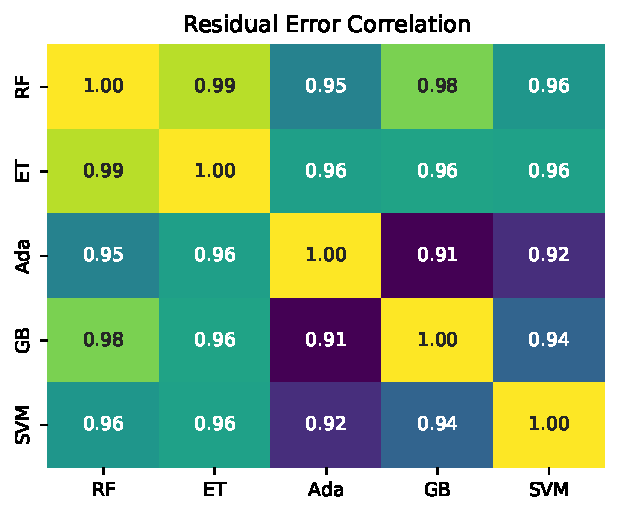
\includegraphics[width=0.32\linewidth]{fig_error_corr.pdf}
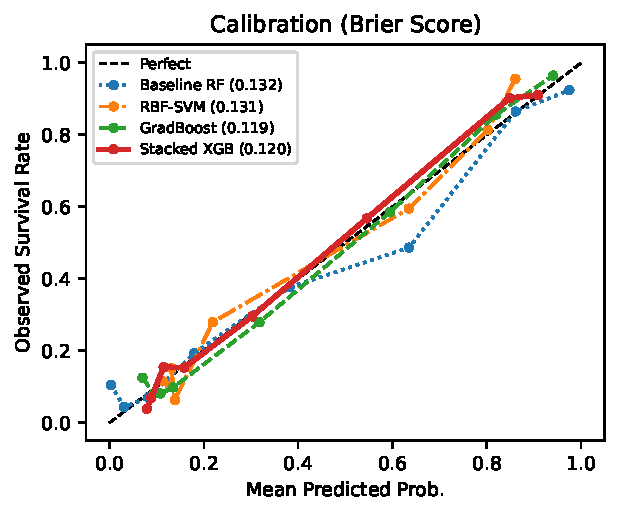
\includegraphics[width=0.32\linewidth]{fig_ablation_cal.pdf}
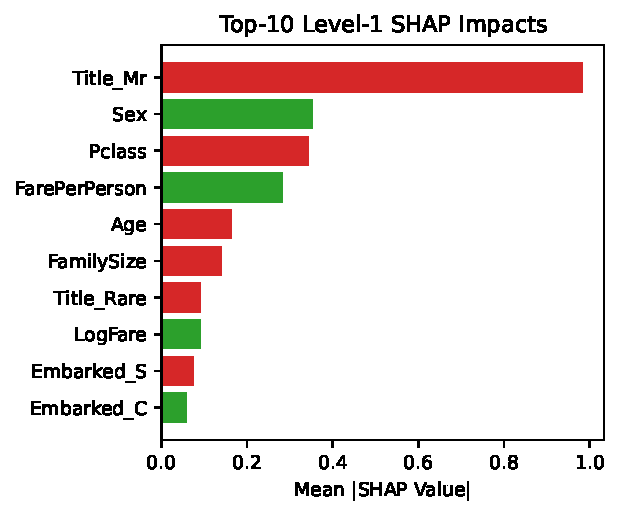
\includegraphics[width=0.32\linewidth]{fig_shap_summary.pdf}
\caption{\textbf{Left:} Residual error correlation across Level-1 models. \textbf{Center:} Reliability calibration curve (Brier score). \textbf{Right:} Top-10 Level-1 SHAP feature impacts (Gradient Boosting).}
\label{fig:depth}
\end{figure}

\section{Limitations and Conclusion}
\textbf{Limitations.} First, $N=891$ training passengers limit statistical power for detecting small accuracy margins. Second, missingness in \texttt{Age} and \texttt{Cabin} is non-random across passenger classes, leaving potential residual bias. Third, Kaggle withholds \texttt{test.csv} ground truth locally (our test predictions yield 156/418 survivors, 91.39\% agreement with \texttt{gender\_submission.csv}). Fourth, SHAP reflects predictive association, not causality; causal claims would require unobserved physical variables (e.g., cabin distance to lifeboats).

\textbf{Conclusion.} A two-level stacked ensemble combining four tree learners and a scaled RBF-SVM via heavily regularized shallow XGBoost achieves 83.16\% 5-fold CV accuracy (+2.02\% above the default Random Forest baseline) and the highest ROC-AUC (0.8902) with strong calibration. Analyzing base-error correlation and meta-learner regularization explains both why ranking/calibration improve and why high inter-model error correlation bounds accuracy gains over the best individual tree ensemble.

\section{Reproducibility and AI-Use Disclosure}
\textbf{Reproducibility.} Code (\texttt{new\_ml\_updated.py}) with fixed seeds (\texttt{SEED=42}) and leak-free \texttt{TitanicPreprocessor} is hosted at \url{https://colab.research.google.com/drive/1u48dL64DrjkH9IoM9S7xI5p6pRicmsEZ} (replace with GitHub URL if preferred). Data is publicly available on Kaggle (\url{https://www.kaggle.com/c/titanic}); running the script reproduces all metrics and \texttt{titanic\_stacked\_submission.csv}. \textbf{AI-Use Disclosure:} Generative AI tools (Gemini / ChatGPT) assisted with diagnostic plot code and LaTeX manuscript formatting; all code execution, outputs, and statistical interpretations were independently verified by the author.

\begin{thebibliography}{9}
\bibitem[Wolpert(1992)]{wolpert1992stacked}
David~H. Wolpert. Stacked generalization. \emph{Neural Networks}, 5(2):241--259, 1992.
\bibitem[Breiman(2001)]{breiman2001random}
Leo Breiman. Random forests. \emph{Machine Learning}, 45(1):5--32, 2001.
\bibitem[Geurts et~al.(2006)]{geurts2006extremely}
Pierre Geurts, Damien Ernst, and Louis Wehenkel. Extremely randomized trees. \emph{Machine Learning}, 63(1):3--42, 2006.
\bibitem[Freund and Schapire(1997)]{freund1997decision}
Yoav Freund and Robert~E. Schapire. A decision-theoretic generalization of on-line learning and an application to boosting. \emph{J. Comput. Syst. Sci.}, 55(1):119--139, 1997.
\bibitem[Friedman(2001)]{friedman2001gradient}
Jerome~H. Friedman. Greedy function approximation: A gradient boosting machine. \emph{Ann. Statist.}, 29(5):1189--1232, 2001.
\bibitem[Cortes and Vapnik(1995)]{cortes1995support}
Corinna Cortes and Vladimir Vapnik. Support-vector networks. \emph{Machine Learning}, 20(3):273--297, 1995.
\bibitem[Chen and Guestrin(2016)]{chen2016xgboost}
Tianqi Chen and Carlos Guestrin. {XGBoost}: A scalable tree boosting system. In \emph{Proc. 22nd ACM SIGKDD}, pages 785--794, 2016.
\bibitem[Lundberg and Lee(2017)]{lundberg2017unified}
Scott~M. Lundberg and Su-In Lee. A unified approach to interpreting model predictions. In \emph{Adv. Neural Inf. Process. Syst. (NeurIPS)}, volume~30, pages 4765--4774, 2017.
\end{thebibliography}

\end{document}
